\documentclass[1p]{elsarticle_modified}
%\bibliographystyle{elsarticle-num}

%\usepackage[colorlinks]{hyperref}
%\usepackage{abbrmath_seonhwa} %\Abb, \Ascr, \Acal ,\Abf, \Afrak
\usepackage{amsfonts}
\usepackage{amssymb}
\usepackage{amsmath}
\usepackage{amsthm}
\usepackage{scalefnt}
\usepackage{amsbsy}
\usepackage{kotex}
\usepackage{caption}
\usepackage{subfig}
\usepackage{color}
\usepackage{graphicx}
\usepackage{xcolor} %% white, black, red, green, blue, cyan, magenta, yellow
\usepackage{float}
\usepackage{setspace}
\usepackage{hyperref}

\usepackage{tikz}
\usetikzlibrary{arrows}

\usepackage{multirow}
\usepackage{array} % fixed length table
\usepackage{hhline}

%%%%%%%%%%%%%%%%%%%%%
\makeatletter
\renewcommand*\env@matrix[1][\arraystretch]{%
	\edef\arraystretch{#1}%
	\hskip -\arraycolsep
	\let\@ifnextchar\new@ifnextchar
	\array{*\c@MaxMatrixCols c}}
\makeatother %https://tex.stackexchange.com/questions/14071/how-can-i-increase-the-line-spacing-in-a-matrix
%%%%%%%%%%%%%%%

\usepackage[normalem]{ulem}

\newcommand{\msout}[1]{\ifmmode\text{\sout{\ensuremath{#1}}}\else\sout{#1}\fi}
%SOURCE: \msout is \stkout macro in https://tex.stackexchange.com/questions/20609/strikeout-in-math-mode

\newcommand{\cancel}[1]{
	\ifmmode
	{\color{red}\msout{#1}}
	\else
	{\color{red}\sout{#1}}
	\fi
}

\newcommand{\add}[1]{
	{\color{blue}\uwave{#1}}
}

\newcommand{\replace}[2]{
	\ifmmode
	{\color{red}\msout{#1}}{\color{blue}\uwave{#2}}
	\else
	{\color{red}\sout{#1}}{\color{blue}\uwave{#2}}
	\fi
}

\newcommand{\Sol}{\mathcal{S}} %segment
\newcommand{\D}{D} %diagram
\newcommand{\A}{\mathcal{A}} %arc


%%%%%%%%%%%%%%%%%%%%%%%%%%%%%5 test

\def\sl{\operatorname{\textup{SL}}(2,\Cbb)}
\def\psl{\operatorname{\textup{PSL}}(2,\Cbb)}
\def\quan{\mkern 1mu \triangleright \mkern 1mu}

\theoremstyle{definition}
\newtheorem{thm}{Theorem}[section]
\newtheorem{prop}[thm]{Proposition}
\newtheorem{lem}[thm]{Lemma}
\newtheorem{ques}[thm]{Question}
\newtheorem{cor}[thm]{Corollary}
\newtheorem{defn}[thm]{Definition}
\newtheorem{exam}[thm]{Example}
\newtheorem{rmk}[thm]{Remark}
\newtheorem{alg}[thm]{Algorithm}

\newcommand{\I}{\sqrt{-1}}
\begin{document}

%\begin{frontmatter}
%
%\title{Boundary parabolic representations of knots up to 8 crossings}
%
%%% Group authors per affiliation:
%\author{Yunhi Cho} 
%\address{Department of Mathematics, University of Seoul, Seoul, Korea}
%\ead{yhcho@uos.ac.kr}
%
%
%\author{Seonhwa Kim} %\fnref{s_kim}}
%\address{Center for Geometry and Physics, Institute for Basic Science, Pohang, 37673, Korea}
%\ead{ryeona17@ibs.re.kr}
%
%\author{Hyuk Kim}
%\address{Department of Mathematical Sciences, Seoul National University, Seoul 08826, Korea}
%\ead{hyukkim@snu.ac.kr}
%
%\author{Seokbeom Yoon}
%\address{Department of Mathematical Sciences, Seoul National University, Seoul, 08826,  Korea}
%\ead{sbyoon15@snu.ac.kr}
%
%\begin{abstract}
%We find all boundary parabolic representation of knots up to 8 crossings.
%
%\end{abstract}
%\begin{keyword}
%    \MSC[2010] 57M25 
%\end{keyword}
%
%\end{frontmatter}

%\linenumbers
%\tableofcontents
%
\newcommand\colored[1]{\textcolor{white}{\rule[-0.35ex]{0.8em}{1.4ex}}\kern-0.8em\color{red} #1}%
%\newcommand\colored[1]{\textcolor{white}{ #1}\kern-2.17ex	\textcolor{white}{ #1}\kern-1.81ex	\textcolor{white}{ #1}\kern-2.15ex\color{red}#1	}

{\Large $\underline{12n_{0156}~(K12n_{0156})}$}

\setlength{\tabcolsep}{10pt}
\renewcommand{\arraystretch}{1.6}
\vspace{1cm}\begin{tabular}{m{100pt}>{\centering\arraybackslash}m{274pt}}
\multirow{5}{120pt}{
	\centering
	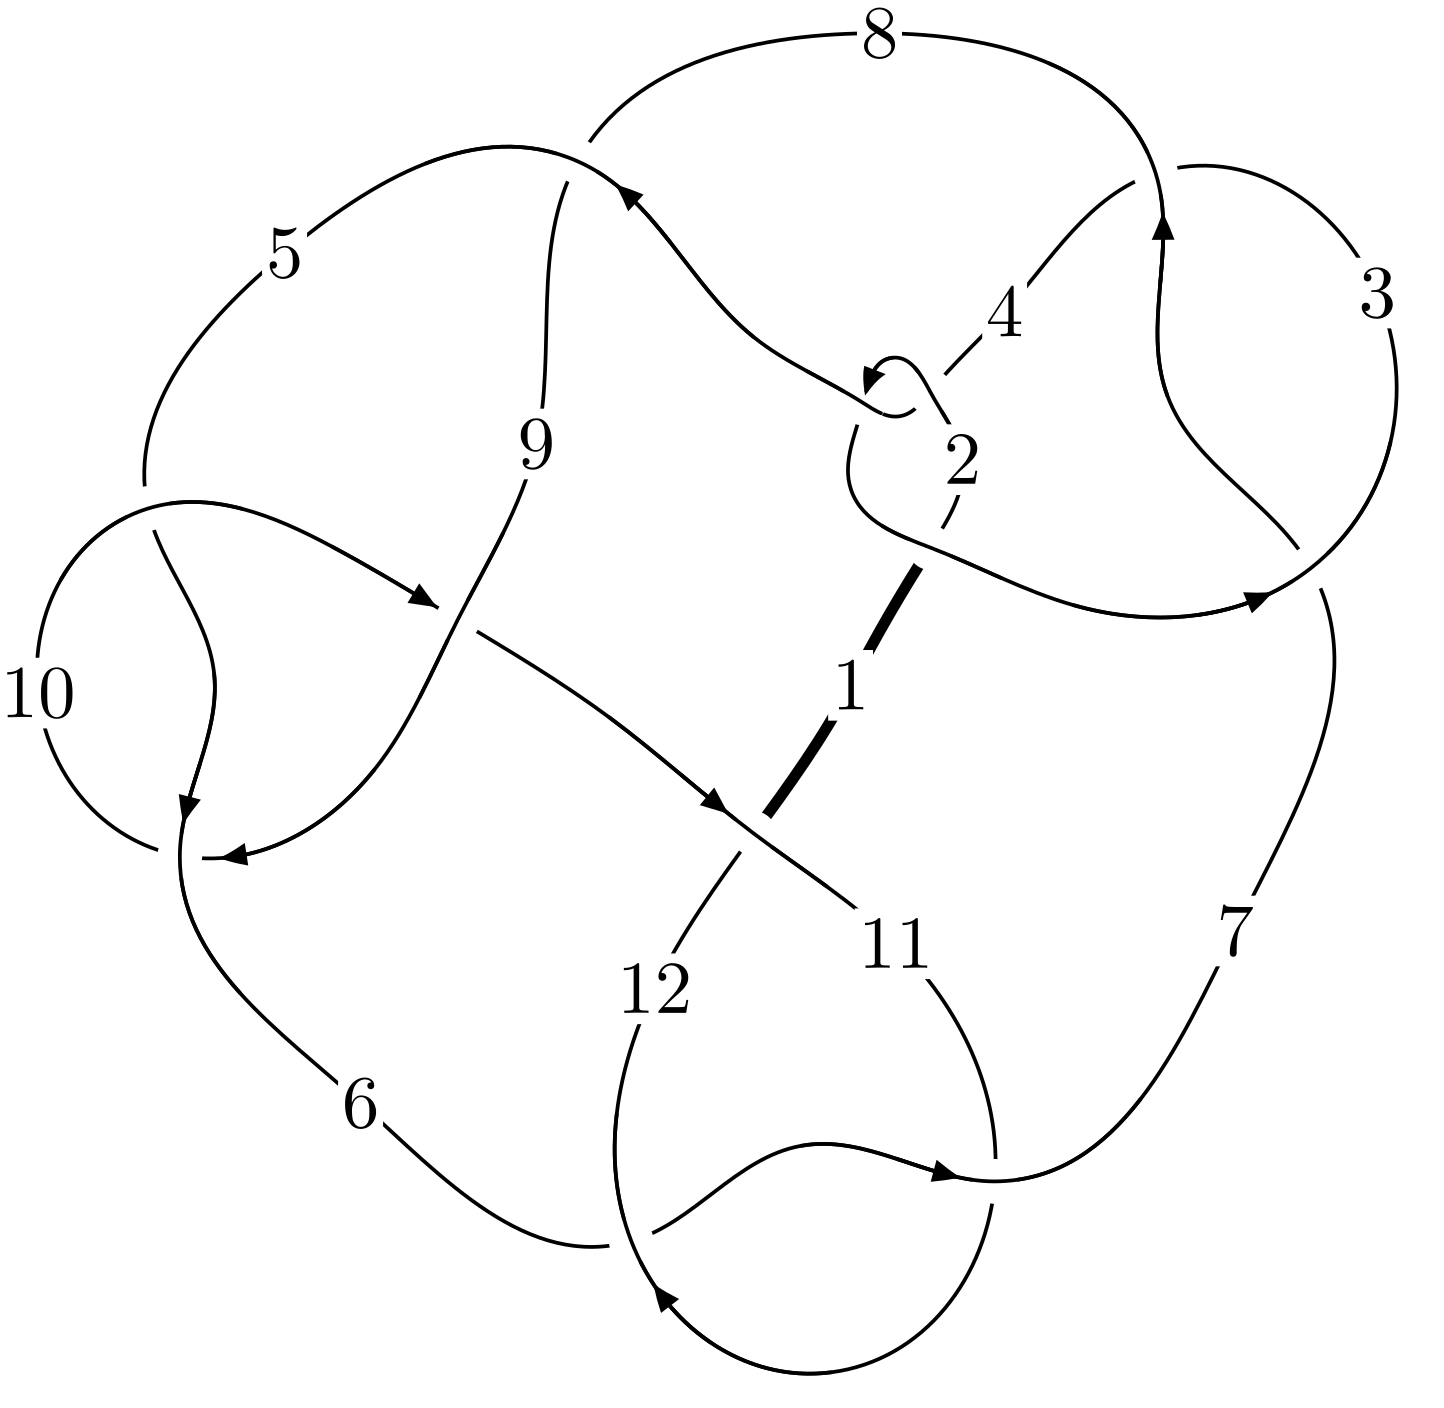
\includegraphics[width=112pt]{../../../GIT/diagram.site/Diagrams/png/2245_12n_0156.png}\\
\ \ \ A knot diagram\footnotemark}&
\allowdisplaybreaks
\textbf{Linearized knot diagam} \\
\cline{2-2}
 &
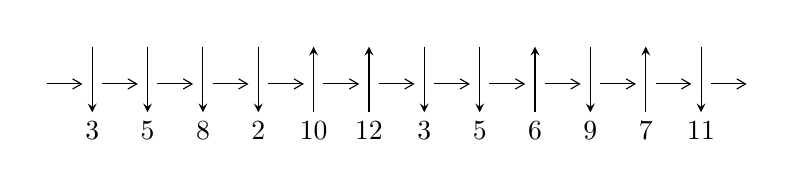
\begin{tikzpicture}[x=20pt, y=17pt]
	% nodes
	\node (C0) at (0, 0) {};
	\node (C1) at (1, 0) {};
	\node (C1U) at (1, +1) {};
	\node (C1D) at (1, -1) {3};

	\node (C2) at (2, 0) {};
	\node (C2U) at (2, +1) {};
	\node (C2D) at (2, -1) {5};

	\node (C3) at (3, 0) {};
	\node (C3U) at (3, +1) {};
	\node (C3D) at (3, -1) {8};

	\node (C4) at (4, 0) {};
	\node (C4U) at (4, +1) {};
	\node (C4D) at (4, -1) {2};

	\node (C5) at (5, 0) {};
	\node (C5U) at (5, +1) {};
	\node (C5D) at (5, -1) {10};

	\node (C6) at (6, 0) {};
	\node (C6U) at (6, +1) {};
	\node (C6D) at (6, -1) {12};

	\node (C7) at (7, 0) {};
	\node (C7U) at (7, +1) {};
	\node (C7D) at (7, -1) {3};

	\node (C8) at (8, 0) {};
	\node (C8U) at (8, +1) {};
	\node (C8D) at (8, -1) {5};

	\node (C9) at (9, 0) {};
	\node (C9U) at (9, +1) {};
	\node (C9D) at (9, -1) {6};

	\node (C10) at (10, 0) {};
	\node (C10U) at (10, +1) {};
	\node (C10D) at (10, -1) {9};

	\node (C11) at (11, 0) {};
	\node (C11U) at (11, +1) {};
	\node (C11D) at (11, -1) {7};

	\node (C12) at (12, 0) {};
	\node (C12U) at (12, +1) {};
	\node (C12D) at (12, -1) {11};
	\node (C13) at (13, 0) {};

	% arrows
	\draw[->,>={angle 60}]
	(C0) edge (C1) (C1) edge (C2) (C2) edge (C3) (C3) edge (C4) (C4) edge (C5) (C5) edge (C6) (C6) edge (C7) (C7) edge (C8) (C8) edge (C9) (C9) edge (C10) (C10) edge (C11) (C11) edge (C12) (C12) edge (C13) ;	\draw[->,>=stealth]
	(C1U) edge (C1D) (C2U) edge (C2D) (C3U) edge (C3D) (C4U) edge (C4D) (C5D) edge (C5U) (C6D) edge (C6U) (C7U) edge (C7D) (C8U) edge (C8D) (C9D) edge (C9U) (C10U) edge (C10D) (C11D) edge (C11U) (C12U) edge (C12D) ;
	\end{tikzpicture} \\
\hhline{~~} \\& 
\textbf{Solving Sequence} \\ \cline{2-2} 
 &
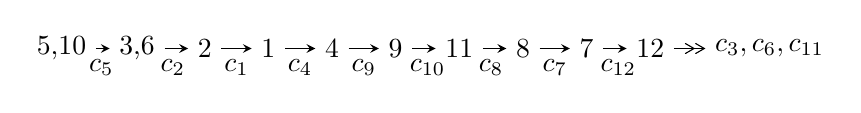
\begin{tikzpicture}[x=23pt, y=7pt]
	% node
	\node (A0) at (-1/8, 0) {5,10};
	\node (A1) at (17/16, 0) {3,6};
	\node (A2) at (17/8, 0) {2};
	\node (A3) at (25/8, 0) {1};
	\node (A4) at (33/8, 0) {4};
	\node (A5) at (41/8, 0) {9};
	\node (A6) at (49/8, 0) {11};
	\node (A7) at (57/8, 0) {8};
	\node (A8) at (65/8, 0) {7};
	\node (A9) at (73/8, 0) {12};
	\node (C1) at (1/2, -1) {$c_{5}$};
	\node (C2) at (13/8, -1) {$c_{2}$};
	\node (C3) at (21/8, -1) {$c_{1}$};
	\node (C4) at (29/8, -1) {$c_{4}$};
	\node (C5) at (37/8, -1) {$c_{9}$};
	\node (C6) at (45/8, -1) {$c_{10}$};
	\node (C7) at (53/8, -1) {$c_{8}$};
	\node (C8) at (61/8, -1) {$c_{7}$};
	\node (C9) at (69/8, -1) {$c_{12}$};
	\node (A10) at (11, 0) {$c_{3},c_{6},c_{11}$};

	% edge
	\draw[->,>=stealth]	
	(A0) edge (A1) (A1) edge (A2) (A2) edge (A3) (A3) edge (A4) (A4) edge (A5) (A5) edge (A6) (A6) edge (A7) (A7) edge (A8) (A8) edge (A9) ;
	\draw[->>,>={angle 60}]	
	(A9) edge (A10);
\end{tikzpicture} \\ 

\end{tabular} \\

\footnotetext{
The image of knot diagram is generated by the software ``\textbf{Draw programme}" developed by Andrew Bartholomew(\url{http://www.layer8.co.uk/maths/draw/index.htm\#Running-draw}), where we modified some parts for our purpose(\url{https://github.com/CATsTAILs/LinksPainter}).
}\phantom \\ \newline 
\centering \textbf{Ideals for irreducible components\footnotemark of $X_{\text{par}}$} 
 
\begin{align*}
I^u_{1}&=\langle 
u^9+u^8+5 u^7+3 u^6+9 u^5+7 u^4+6 u^3+5 u^2+4 b+3,\\
\phantom{I^u_{1}}&\phantom{= \langle  }- u^9+3 u^8-5 u^7+5 u^6-5 u^5+u^4+2 u^3-13 u^2+8 a+8 u-11,\\
\phantom{I^u_{1}}&\phantom{= \langle  }u^{10}+4 u^8+2 u^7+6 u^6+6 u^5+3 u^4+7 u^3- u^2+3 u+1\rangle \\
I^u_{2}&=\langle 
b+1,\;- u^3+u^2+2 a+1,\;u^4+u^2+u+1\rangle \\
I^u_{3}&=\langle 
-4 u^{15}+18 u^{14}+\cdots+33 b+38,\;29 u^{15}-48 u^{14}+\cdots+33 a-61,\;u^{16}-2 u^{15}+\cdots-2 u+1\rangle \\
I^u_{4}&=\langle 
b+1,\;u^5- u^4+u^3- u^2+a+u,\;u^6- u^5+2 u^4-2 u^3+2 u^2-2 u+1\rangle \\
\\
\end{align*}
\raggedright * 4 irreducible components of $\dim_{\mathbb{C}}=0$, with total 36 representations.\\
\footnotetext{All coefficients of polynomials are rational numbers. But the coefficients are sometimes approximated in decimal forms when there is not enough margin.}
\newpage
\renewcommand{\arraystretch}{1}
\centering \section*{I. $I^u_{1}= \langle u^9+u^8+\cdots+4 b+3,\;- u^9+3 u^8+\cdots+8 a-11,\;u^{10}+4 u^8+\cdots+3 u+1 \rangle$}
\flushleft \textbf{(i) Arc colorings}\\
\begin{tabular}{m{7pt} m{180pt} m{7pt} m{180pt} }
\flushright $a_{5}=$&$\begin{pmatrix}1\\0\end{pmatrix}$ \\
\flushright $a_{10}=$&$\begin{pmatrix}0\\u\end{pmatrix}$ \\
\flushright $a_{3}=$&$\begin{pmatrix}\frac{1}{8} u^9-\frac{3}{8} u^8+\cdots- u+\frac{11}{8}\\-\frac{1}{4} u^9-\frac{1}{4} u^8+\cdots-\frac{5}{4} u^2-\frac{3}{4}\end{pmatrix}$ \\
\flushright $a_{6}=$&$\begin{pmatrix}1\\- u^2\end{pmatrix}$ \\
\flushright $a_{2}=$&$\begin{pmatrix}-\frac{1}{8} u^9-\frac{5}{8} u^8+\cdots- u+\frac{5}{8}\\-\frac{1}{4} u^9-\frac{1}{4} u^8+\cdots-\frac{5}{4} u^2-\frac{3}{4}\end{pmatrix}$ \\
\flushright $a_{1}=$&$\begin{pmatrix}- u^9-3 u^7-2 u^6-4 u^5-4 u^4-3 u^2\\- u^9-2 u^7-2 u^6-2 u^5-4 u^4+2 u^3-3 u^2\end{pmatrix}$ \\
\flushright $a_{4}=$&$\begin{pmatrix}\frac{13}{8} u^9-\frac{7}{8} u^8+\cdots-2 u+\frac{7}{8}\\\frac{3}{4} u^9-\frac{1}{4} u^8+\cdots+\frac{3}{4} u^2-\frac{3}{4}\end{pmatrix}$ \\
\flushright $a_{9}=$&$\begin{pmatrix}- u\\u^3+u\end{pmatrix}$ \\
\flushright $a_{11}=$&$\begin{pmatrix}- u^3\\u^5+u^3+u\end{pmatrix}$ \\
\flushright $a_{8}=$&$\begin{pmatrix}u^3\\u^3+u\end{pmatrix}$ \\
\flushright $a_{7}=$&$\begin{pmatrix}u^8+3 u^6+2 u^5+3 u^4+4 u^3- u^2+3 u\\u^8+3 u^6+2 u^5+4 u^4+4 u^3+3 u+1\end{pmatrix}$ \\
\flushright $a_{12}=$&$\begin{pmatrix}- u^9-3 u^7-2 u^6-3 u^5-4 u^4-3 u^2\\- u^9-3 u^7-2 u^6-3 u^5-4 u^4+u^3-3 u^2\end{pmatrix}$\\&\end{tabular}
\flushleft \textbf{(ii) Obstruction class $= -1$}\\~\\
\flushleft \textbf{(iii) Cusp Shapes $= -\frac{33}{16} u^9-\frac{53}{16} u^8-\frac{141}{16} u^7-\frac{227}{16} u^6-\frac{325}{16} u^5-\frac{367}{16} u^4-\frac{159}{8} u^3-\frac{237}{16} u^2-6 u-\frac{147}{16}$}\\~\\
\newpage\renewcommand{\arraystretch}{1}
\flushleft \textbf{(iv) u-Polynomials at the component}\newline \\
\begin{tabular}{m{50pt}|m{274pt}}
Crossings & \hspace{64pt}u-Polynomials at each crossing \\
\hline $$\begin{aligned}c_{1}\end{aligned}$$&$\begin{aligned}
&u^{10}+17 u^9+\cdots+353 u+16
\end{aligned}$\\
\hline $$\begin{aligned}c_{2},c_{4}\end{aligned}$$&$\begin{aligned}
&u^{10}-3 u^9-4 u^8+13 u^7+22 u^6-70 u^5+56 u^4-7 u^3-47 u^2+27 u-4
\end{aligned}$\\
\hline $$\begin{aligned}c_{3},c_{7}\end{aligned}$$&$\begin{aligned}
&u^{10}-3 u^9+\cdots-48 u-64
\end{aligned}$\\
\hline $$\begin{aligned}c_{5},c_{6},c_{9}\\c_{11}\end{aligned}$$&$\begin{aligned}
&u^{10}+4 u^8+2 u^7+6 u^6+6 u^5+3 u^4+7 u^3- u^2+3 u+1
\end{aligned}$\\
\hline $$\begin{aligned}c_{8}\end{aligned}$$&$\begin{aligned}
&u^{10}+6 u^9+9 u^8-6 u^7-21 u^6-14 u^5+21 u^3+13 u^2+16 u+4
\end{aligned}$\\
\hline $$\begin{aligned}c_{10},c_{12}\end{aligned}$$&$\begin{aligned}
&u^{10}+8 u^9+\cdots-11 u+1
\end{aligned}$\\
\hline
\end{tabular}\\~\\
\newpage\renewcommand{\arraystretch}{1}
\flushleft \textbf{(v) Riley Polynomials at the component}\newline \\
\begin{tabular}{m{50pt}|m{274pt}}
Crossings & \hspace{64pt}Riley Polynomials at each crossing \\
\hline $$\begin{aligned}c_{1}\end{aligned}$$&$\begin{aligned}
&y^{10}-13 y^9+\cdots-56161 y+256
\end{aligned}$\\
\hline $$\begin{aligned}c_{2},c_{4}\end{aligned}$$&$\begin{aligned}
&y^{10}-17 y^9+\cdots-353 y+16
\end{aligned}$\\
\hline $$\begin{aligned}c_{3},c_{7}\end{aligned}$$&$\begin{aligned}
&y^{10}-21 y^9+\cdots+16128 y+4096
\end{aligned}$\\
\hline $$\begin{aligned}c_{5},c_{6},c_{9}\\c_{11}\end{aligned}$$&$\begin{aligned}
&y^{10}+8 y^9+\cdots-11 y+1
\end{aligned}$\\
\hline $$\begin{aligned}c_{8}\end{aligned}$$&$\begin{aligned}
&y^{10}-18 y^9+\cdots-152 y+16
\end{aligned}$\\
\hline $$\begin{aligned}c_{10},c_{12}\end{aligned}$$&$\begin{aligned}
&y^{10}-8 y^9+\cdots-191 y+1
\end{aligned}$\\
\hline
\end{tabular}\\~\\
\newpage\flushleft \textbf{(vi) Complex Volumes and Cusp Shapes}
$$\begin{array}{c|c|c}  
\text{Solutions to }I^u_{1}& \I (\text{vol} + \sqrt{-1}CS) & \text{Cusp shape}\\
 \hline 
\begin{aligned}
u &= -1.10322\phantom{ +0.000000I} \\
a &= \phantom{-}0.0897722\phantom{ +0.000000I} \\
b &= \phantom{-}2.01806\phantom{ +0.000000I}\end{aligned}
 & -13.1809\phantom{ +0.000000I} & -5.01890\phantom{ +0.000000I} \\ \hline\begin{aligned}
u &= -0.434341 + 1.157890 I \\
a &= \phantom{-}0.168075 - 0.547483 I \\
b &= \phantom{-}0.424180 - 0.920028 I\end{aligned}
 & -3.22150 - 6.17796 I & -7.18871 + 5.57381 I \\ \hline\begin{aligned}
u &= -0.434341 - 1.157890 I \\
a &= \phantom{-}0.168075 + 0.547483 I \\
b &= \phantom{-}0.424180 + 0.920028 I\end{aligned}
 & -3.22150 + 6.17796 I & -7.18871 - 5.57381 I \\ \hline\begin{aligned}
u &= \phantom{-}0.453609 + 0.609493 I \\
a &= \phantom{-}0.755807 + 0.185749 I \\
b &= \phantom{-}0.306434 - 0.019942 I\end{aligned}
 & \phantom{-}0.54459 + 1.46281 I & \phantom{-}2.01320 - 4.52195 I \\ \hline\begin{aligned}
u &= \phantom{-}0.453609 - 0.609493 I \\
a &= \phantom{-}0.755807 - 0.185749 I \\
b &= \phantom{-}0.306434 + 0.019942 I\end{aligned}
 & \phantom{-}0.54459 - 1.46281 I & \phantom{-}2.01320 + 4.52195 I \\ \hline\begin{aligned}
u &= \phantom{-}0.126773 + 1.317690 I \\
a &= -1.87389 + 0.33187 I \\
b &= -1.95902 + 1.19918 I\end{aligned}
 & -9.42139 + 3.00890 I & -13.74651 - 2.98751 I \\ \hline\begin{aligned}
u &= \phantom{-}0.126773 - 1.317690 I \\
a &= -1.87389 - 0.33187 I \\
b &= -1.95902 - 1.19918 I\end{aligned}
 & -9.42139 - 3.00890 I & -13.74651 + 2.98751 I \\ \hline\begin{aligned}
u &= \phantom{-}0.53944 + 1.37745 I \\
a &= \phantom{-}1.77401 + 1.11600 I \\
b &= \phantom{-}2.12782 - 0.47355 I\end{aligned}
 & \phantom{-}17.6402 + 11.6714 I & -10.01565 - 5.34252 I \\ \hline\begin{aligned}
u &= \phantom{-}0.53944 - 1.37745 I \\
a &= \phantom{-}1.77401 - 1.11600 I \\
b &= \phantom{-}2.12782 + 0.47355 I\end{aligned}
 & \phantom{-}17.6402 - 11.6714 I & -10.01565 + 5.34252 I \\ \hline\begin{aligned}
u &= -0.267745\phantom{ +0.000000I} \\
a &= \phantom{-}1.76223\phantom{ +0.000000I} \\
b &= -0.816874\phantom{ +0.000000I}\end{aligned}
 & -1.19281\phantom{ +0.000000I} & -8.35580\phantom{ +0.000000I}\\
 \hline 
 \end{array}$$\newpage\newpage\renewcommand{\arraystretch}{1}
\centering \section*{II. $I^u_{2}= \langle b+1,\;- u^3+u^2+2 a+1,\;u^4+u^2+u+1 \rangle$}
\flushleft \textbf{(i) Arc colorings}\\
\begin{tabular}{m{7pt} m{180pt} m{7pt} m{180pt} }
\flushright $a_{5}=$&$\begin{pmatrix}1\\0\end{pmatrix}$ \\
\flushright $a_{10}=$&$\begin{pmatrix}0\\u\end{pmatrix}$ \\
\flushright $a_{3}=$&$\begin{pmatrix}\frac{1}{2} u^3-\frac{1}{2} u^2-\frac{1}{2}\\-1\end{pmatrix}$ \\
\flushright $a_{6}=$&$\begin{pmatrix}1\\- u^2\end{pmatrix}$ \\
\flushright $a_{2}=$&$\begin{pmatrix}\frac{1}{2} u^3-\frac{1}{2} u^2-\frac{3}{2}\\-1\end{pmatrix}$ \\
\flushright $a_{1}=$&$\begin{pmatrix}-1\\0\end{pmatrix}$ \\
\flushright $a_{4}=$&$\begin{pmatrix}\frac{1}{2} u^3-\frac{1}{2} u^2-\frac{1}{2}\\-1\end{pmatrix}$ \\
\flushright $a_{9}=$&$\begin{pmatrix}- u\\u^3+u\end{pmatrix}$ \\
\flushright $a_{11}=$&$\begin{pmatrix}- u^3\\- u^2\end{pmatrix}$ \\
\flushright $a_{8}=$&$\begin{pmatrix}u^3\\u^3+u\end{pmatrix}$ \\
\flushright $a_{7}=$&$\begin{pmatrix}u^3\\u^3+u\end{pmatrix}$ \\
\flushright $a_{12}=$&$\begin{pmatrix}- u^3- u^2- u-1\\- u^2- u-1\end{pmatrix}$\\&\end{tabular}
\flushleft \textbf{(ii) Obstruction class $= 1$}\\~\\
\flushleft \textbf{(iii) Cusp Shapes $= \frac{11}{4} u^3-\frac{21}{4} u^2-\frac{1}{2} u-\frac{31}{4}$}\\~\\
\newpage\renewcommand{\arraystretch}{1}
\flushleft \textbf{(iv) u-Polynomials at the component}\newline \\
\begin{tabular}{m{50pt}|m{274pt}}
Crossings & \hspace{64pt}u-Polynomials at each crossing \\
\hline $$\begin{aligned}c_{1},c_{2}\end{aligned}$$&$\begin{aligned}
&(u-1)^4
\end{aligned}$\\
\hline $$\begin{aligned}c_{3},c_{7}\end{aligned}$$&$\begin{aligned}
&u^4
\end{aligned}$\\
\hline $$\begin{aligned}c_{4}\end{aligned}$$&$\begin{aligned}
&(u+1)^4
\end{aligned}$\\
\hline $$\begin{aligned}c_{5},c_{6}\end{aligned}$$&$\begin{aligned}
&u^4+u^2+u+1
\end{aligned}$\\
\hline $$\begin{aligned}c_{8}\end{aligned}$$&$\begin{aligned}
&u^4-3 u^3+4 u^2-3 u+2
\end{aligned}$\\
\hline $$\begin{aligned}c_{9},c_{11}\end{aligned}$$&$\begin{aligned}
&u^4+u^2- u+1
\end{aligned}$\\
\hline $$\begin{aligned}c_{10},c_{12}\end{aligned}$$&$\begin{aligned}
&u^4+2 u^3+3 u^2+u+1
\end{aligned}$\\
\hline
\end{tabular}\\~\\
\newpage\renewcommand{\arraystretch}{1}
\flushleft \textbf{(v) Riley Polynomials at the component}\newline \\
\begin{tabular}{m{50pt}|m{274pt}}
Crossings & \hspace{64pt}Riley Polynomials at each crossing \\
\hline $$\begin{aligned}c_{1},c_{2},c_{4}\end{aligned}$$&$\begin{aligned}
&(y-1)^4
\end{aligned}$\\
\hline $$\begin{aligned}c_{3},c_{7}\end{aligned}$$&$\begin{aligned}
&y^4
\end{aligned}$\\
\hline $$\begin{aligned}c_{5},c_{6},c_{9}\\c_{11}\end{aligned}$$&$\begin{aligned}
&y^4+2 y^3+3 y^2+y+1
\end{aligned}$\\
\hline $$\begin{aligned}c_{8}\end{aligned}$$&$\begin{aligned}
&y^4- y^3+2 y^2+7 y+4
\end{aligned}$\\
\hline $$\begin{aligned}c_{10},c_{12}\end{aligned}$$&$\begin{aligned}
&y^4+2 y^3+7 y^2+5 y+1
\end{aligned}$\\
\hline
\end{tabular}\\~\\
\newpage\flushleft \textbf{(vi) Complex Volumes and Cusp Shapes}
$$\begin{array}{c|c|c}  
\text{Solutions to }I^u_{2}& \I (\text{vol} + \sqrt{-1}CS) & \text{Cusp shape}\\
 \hline 
\begin{aligned}
u &= -0.547424 + 0.585652 I \\
a &= -0.278726 + 0.483420 I \\
b &= -1.00000\phantom{ +0.000000I}\end{aligned}
 & -0.66484 - 1.39709 I & -6.15099 + 3.96898 I \\ \hline\begin{aligned}
u &= -0.547424 - 0.585652 I \\
a &= -0.278726 - 0.483420 I \\
b &= -1.00000\phantom{ +0.000000I}\end{aligned}
 & -0.66484 + 1.39709 I & -6.15099 - 3.96898 I \\ \hline\begin{aligned}
u &= \phantom{-}0.547424 + 1.120870 I \\
a &= -0.971274 - 0.813859 I \\
b &= -1.00000\phantom{ +0.000000I}\end{aligned}
 & -4.26996 + 7.64338 I & -8.22401 - 8.10462 I \\ \hline\begin{aligned}
u &= \phantom{-}0.547424 - 1.120870 I \\
a &= -0.971274 + 0.813859 I \\
b &= -1.00000\phantom{ +0.000000I}\end{aligned}
 & -4.26996 - 7.64338 I & -8.22401 + 8.10462 I\\
 \hline 
 \end{array}$$\newpage\newpage\renewcommand{\arraystretch}{1}
\centering \section*{III. $I^u_{3}= \langle -4 u^{15}+18 u^{14}+\cdots+33 b+38,\;29 u^{15}-48 u^{14}+\cdots+33 a-61,\;u^{16}-2 u^{15}+\cdots-2 u+1 \rangle$}
\flushleft \textbf{(i) Arc colorings}\\
\begin{tabular}{m{7pt} m{180pt} m{7pt} m{180pt} }
\flushright $a_{5}=$&$\begin{pmatrix}1\\0\end{pmatrix}$ \\
\flushright $a_{10}=$&$\begin{pmatrix}0\\u\end{pmatrix}$ \\
\flushright $a_{3}=$&$\begin{pmatrix}-0.878788 u^{15}+1.45455 u^{14}+\cdots-0.636364 u+1.84848\\0.121212 u^{15}-0.545455 u^{14}+\cdots+0.363636 u-1.15152\end{pmatrix}$ \\
\flushright $a_{6}=$&$\begin{pmatrix}1\\- u^2\end{pmatrix}$ \\
\flushright $a_{2}=$&$\begin{pmatrix}-0.757576 u^{15}+0.909091 u^{14}+\cdots-0.272727 u+0.696970\\0.121212 u^{15}-0.545455 u^{14}+\cdots+0.363636 u-1.15152\end{pmatrix}$ \\
\flushright $a_{1}=$&$\begin{pmatrix}1.27273 u^{15}-2.72727 u^{14}+\cdots+3.81818 u-2.09091\\1.78788 u^{15}-1.54545 u^{14}+\cdots+0.363636 u-1.48485\end{pmatrix}$ \\
\flushright $a_{4}=$&$\begin{pmatrix}-0.393939 u^{15}+1.27273 u^{14}+\cdots-0.181818 u+1.24242\\1.36364 u^{15}-1.63636 u^{14}+\cdots+2.09091 u-2.45455\end{pmatrix}$ \\
\flushright $a_{9}=$&$\begin{pmatrix}- u\\u^3+u\end{pmatrix}$ \\
\flushright $a_{11}=$&$\begin{pmatrix}- u^3\\u^5+u^3+u\end{pmatrix}$ \\
\flushright $a_{8}=$&$\begin{pmatrix}u^3\\u^3+u\end{pmatrix}$ \\
\flushright $a_{7}=$&$\begin{pmatrix}-0.0909091 u^{15}-0.0909091 u^{14}+\cdots+2.72727 u+1.36364\\1.21212 u^{15}-1.45455 u^{14}+\cdots+1.63636 u-2.51515\end{pmatrix}$ \\
\flushright $a_{12}=$&$\begin{pmatrix}2.24242 u^{15}-3.09091 u^{14}+\cdots+4.72727 u-3.30303\\-2.75758 u^{15}+2.90909 u^{14}+\cdots-3.27273 u+2.69697\end{pmatrix}$\\&\end{tabular}
\flushleft \textbf{(ii) Obstruction class $= -1$}\\~\\
\flushleft \textbf{(iii) Cusp Shapes $= -\frac{19}{11} u^{15}+\frac{25}{11} u^{14}-\frac{135}{11} u^{13}+\frac{153}{11} u^{12}-\frac{410}{11} u^{11}+\frac{412}{11} u^{10}-\frac{603}{11} u^9+\frac{543}{11} u^8-29 u^7+\frac{303}{11} u^6+\frac{127}{11} u^5+\frac{60}{11} u^4+\frac{67}{11} u^3+\frac{56}{11} u^2-\frac{90}{11} u-\frac{34}{11}$}\\~\\
\newpage\renewcommand{\arraystretch}{1}
\flushleft \textbf{(iv) u-Polynomials at the component}\newline \\
\begin{tabular}{m{50pt}|m{274pt}}
Crossings & \hspace{64pt}u-Polynomials at each crossing \\
\hline $$\begin{aligned}c_{1}\end{aligned}$$&$\begin{aligned}
&(u^8+16 u^7+98 u^6+283 u^5+381 u^4+191 u^3-45 u^2+10 u+1)^2
\end{aligned}$\\
\hline $$\begin{aligned}c_{2},c_{4}\end{aligned}$$&$\begin{aligned}
&(u^8-4 u^7+13 u^5-3 u^4-15 u^3+3 u^2-2 u-1)^2
\end{aligned}$\\
\hline $$\begin{aligned}c_{3},c_{7}\end{aligned}$$&$\begin{aligned}
&(u^8+u^7-10 u^6-7 u^5+19 u^4-23 u^3-12 u+8)^2
\end{aligned}$\\
\hline $$\begin{aligned}c_{5},c_{6},c_{9}\\c_{11}\end{aligned}$$&$\begin{aligned}
&u^{16}-2 u^{15}+\cdots-2 u+1
\end{aligned}$\\
\hline $$\begin{aligned}c_{8}\end{aligned}$$&$\begin{aligned}
&(u^8-2 u^7-7 u^6+12 u^5+7 u^4-2 u^3-2 u^2+3 u-1)^2
\end{aligned}$\\
\hline $$\begin{aligned}c_{10},c_{12}\end{aligned}$$&$\begin{aligned}
&u^{16}+10 u^{15}+\cdots+14 u^2+1
\end{aligned}$\\
\hline
\end{tabular}\\~\\
\newpage\renewcommand{\arraystretch}{1}
\flushleft \textbf{(v) Riley Polynomials at the component}\newline \\
\begin{tabular}{m{50pt}|m{274pt}}
Crossings & \hspace{64pt}Riley Polynomials at each crossing \\
\hline $$\begin{aligned}c_{1}\end{aligned}$$&$\begin{aligned}
&(y^8-60 y^7+\cdots-190 y+1)^{2}
\end{aligned}$\\
\hline $$\begin{aligned}c_{2},c_{4}\end{aligned}$$&$\begin{aligned}
&(y^8-16 y^7+98 y^6-283 y^5+381 y^4-191 y^3-45 y^2-10 y+1)^2
\end{aligned}$\\
\hline $$\begin{aligned}c_{3},c_{7}\end{aligned}$$&$\begin{aligned}
&(y^8-21 y^7+152 y^6-383 y^5+79 y^4-857 y^3-248 y^2-144 y+64)^2
\end{aligned}$\\
\hline $$\begin{aligned}c_{5},c_{6},c_{9}\\c_{11}\end{aligned}$$&$\begin{aligned}
&y^{16}+10 y^{15}+\cdots+14 y^2+1
\end{aligned}$\\
\hline $$\begin{aligned}c_{8}\end{aligned}$$&$\begin{aligned}
&(y^8-18 y^7+111 y^6-254 y^5+135 y^4-90 y^3+2 y^2-5 y+1)^2
\end{aligned}$\\
\hline $$\begin{aligned}c_{10},c_{12}\end{aligned}$$&$\begin{aligned}
&y^{16}-10 y^{15}+\cdots+28 y+1
\end{aligned}$\\
\hline
\end{tabular}\\~\\
\newpage\flushleft \textbf{(vi) Complex Volumes and Cusp Shapes}
$$\begin{array}{c|c|c}  
\text{Solutions to }I^u_{3}& \I (\text{vol} + \sqrt{-1}CS) & \text{Cusp shape}\\
 \hline 
\begin{aligned}
u &= \phantom{-}0.381176 + 0.988501 I \\
a &= \phantom{-}0.400335 + 0.134981 I \\
b &= \phantom{-}0.202560 + 0.429200 I\end{aligned}
 & -0.54882 + 2.12062 I & -1.41411 - 2.85603 I \\ \hline\begin{aligned}
u &= \phantom{-}0.381176 - 0.988501 I \\
a &= \phantom{-}0.400335 - 0.134981 I \\
b &= \phantom{-}0.202560 - 0.429200 I\end{aligned}
 & -0.54882 - 2.12062 I & -1.41411 + 2.85603 I \\ \hline\begin{aligned}
u &= -0.175038 + 1.044950 I \\
a &= \phantom{-}0.881139 + 0.709579 I \\
b &= -0.266855\phantom{ +0.000000I}\end{aligned}
 & -3.96569\phantom{ +0.000000I} & -10.71257 + 0. I\phantom{ +0.000000I} \\ \hline\begin{aligned}
u &= -0.175038 - 1.044950 I \\
a &= \phantom{-}0.881139 - 0.709579 I \\
b &= -0.266855\phantom{ +0.000000I}\end{aligned}
 & -3.96569\phantom{ +0.000000I} & -10.71257 + 0. I\phantom{ +0.000000I} \\ \hline\begin{aligned}
u &= \phantom{-}1.097050 + 0.006514 I \\
a &= \phantom{-}0.0528548 + 0.1140410 I \\
b &= \phantom{-}2.08865 - 0.23775 I\end{aligned}
 & -17.5075 + 5.8605 I & -7.51154 - 2.72065 I \\ \hline\begin{aligned}
u &= \phantom{-}1.097050 - 0.006514 I \\
a &= \phantom{-}0.0528548 - 0.1140410 I \\
b &= \phantom{-}2.08865 + 0.23775 I\end{aligned}
 & -17.5075 - 5.8605 I & -7.51154 + 2.72065 I \\ \hline\begin{aligned}
u &= -0.087856 + 1.180370 I \\
a &= -1.94399 + 0.56029 I \\
b &= -1.251300 - 0.394571 I\end{aligned}
 & -4.42998 - 1.32248 I & -7.15537 + 1.48485 I \\ \hline\begin{aligned}
u &= -0.087856 - 1.180370 I \\
a &= -1.94399 - 0.56029 I \\
b &= -1.251300 + 0.394571 I\end{aligned}
 & -4.42998 + 1.32248 I & -7.15537 - 1.48485 I \\ \hline\begin{aligned}
u &= -0.579676 + 0.232048 I \\
a &= \phantom{-}0.915955 - 0.352378 I \\
b &= \phantom{-}0.202560 + 0.429200 I\end{aligned}
 & -0.54882 + 2.12062 I & -1.41411 - 2.85603 I \\ \hline\begin{aligned}
u &= -0.579676 - 0.232048 I \\
a &= \phantom{-}0.915955 + 0.352378 I \\
b &= \phantom{-}0.202560 - 0.429200 I\end{aligned}
 & -0.54882 - 2.12062 I & -1.41411 + 2.85603 I\\
 \hline 
 \end{array}$$\newpage$$\begin{array}{c|c|c}  
\text{Solutions to }I^u_{3}& \I (\text{vol} + \sqrt{-1}CS) & \text{Cusp shape}\\
 \hline 
\begin{aligned}
u &= \phantom{-}0.54916 + 1.38012 I \\
a &= \phantom{-}1.49564 + 1.24562 I \\
b &= \phantom{-}2.18705\phantom{ +0.000000I}\end{aligned}
 & \phantom{-}17.6846\phantom{ +0.000000I} & -10.12539 + 0. I\phantom{ +0.000000I} \\ \hline\begin{aligned}
u &= \phantom{-}0.54916 - 1.38012 I \\
a &= \phantom{-}1.49564 - 1.24562 I \\
b &= \phantom{-}2.18705\phantom{ +0.000000I}\end{aligned}
 & \phantom{-}17.6846\phantom{ +0.000000I} & -10.12539 + 0. I\phantom{ +0.000000I} \\ \hline\begin{aligned}
u &= -0.54464 + 1.38261 I \\
a &= \phantom{-}1.62067 - 1.13338 I \\
b &= \phantom{-}2.08865 + 0.23775 I\end{aligned}
 & -17.5075 - 5.8605 I & -7.51154 + 2.72065 I \\ \hline\begin{aligned}
u &= -0.54464 - 1.38261 I \\
a &= \phantom{-}1.62067 + 1.13338 I \\
b &= \phantom{-}2.08865 - 0.23775 I\end{aligned}
 & -17.5075 + 5.8605 I & -7.51154 - 2.72065 I \\ \hline\begin{aligned}
u &= \phantom{-}0.359826 + 0.343977 I \\
a &= \phantom{-}2.07740 - 0.65398 I \\
b &= -1.251300 + 0.394571 I\end{aligned}
 & -4.42998 + 1.32248 I & -7.15537 - 1.48485 I \\ \hline\begin{aligned}
u &= \phantom{-}0.359826 - 0.343977 I \\
a &= \phantom{-}2.07740 + 0.65398 I \\
b &= -1.251300 - 0.394571 I\end{aligned}
 & -4.42998 - 1.32248 I & -7.15537 + 1.48485 I\\
 \hline 
 \end{array}$$\newpage\newpage\renewcommand{\arraystretch}{1}
\centering \section*{IV. $I^u_{4}= \langle b+1,\;u^5- u^4+u^3- u^2+a+u,\;u^6- u^5+2 u^4-2 u^3+2 u^2-2 u+1 \rangle$}
\flushleft \textbf{(i) Arc colorings}\\
\begin{tabular}{m{7pt} m{180pt} m{7pt} m{180pt} }
\flushright $a_{5}=$&$\begin{pmatrix}1\\0\end{pmatrix}$ \\
\flushright $a_{10}=$&$\begin{pmatrix}0\\u\end{pmatrix}$ \\
\flushright $a_{3}=$&$\begin{pmatrix}- u^5+u^4- u^3+u^2- u\\-1\end{pmatrix}$ \\
\flushright $a_{6}=$&$\begin{pmatrix}1\\- u^2\end{pmatrix}$ \\
\flushright $a_{2}=$&$\begin{pmatrix}- u^5+u^4- u^3+u^2- u-1\\-1\end{pmatrix}$ \\
\flushright $a_{1}=$&$\begin{pmatrix}-1\\0\end{pmatrix}$ \\
\flushright $a_{4}=$&$\begin{pmatrix}- u^5+u^4- u^3+u^2- u\\-1\end{pmatrix}$ \\
\flushright $a_{9}=$&$\begin{pmatrix}- u\\u^3+u\end{pmatrix}$ \\
\flushright $a_{11}=$&$\begin{pmatrix}- u^3\\u^5+u^3+u\end{pmatrix}$ \\
\flushright $a_{8}=$&$\begin{pmatrix}u^3\\u^3+u\end{pmatrix}$ \\
\flushright $a_{7}=$&$\begin{pmatrix}u^3\\u^3+u\end{pmatrix}$ \\
\flushright $a_{12}=$&$\begin{pmatrix}- u^4- u^2+u-1\\2 u^5- u^4+3 u^3-2 u^2+3 u-2\end{pmatrix}$\\&\end{tabular}
\flushleft \textbf{(ii) Obstruction class $= 1$}\\~\\
\flushleft \textbf{(iii) Cusp Shapes $= u^5+5 u^3- u^2+5 u-10$}\\~\\
\newpage\renewcommand{\arraystretch}{1}
\flushleft \textbf{(iv) u-Polynomials at the component}\newline \\
\begin{tabular}{m{50pt}|m{274pt}}
Crossings & \hspace{64pt}u-Polynomials at each crossing \\
\hline $$\begin{aligned}c_{1},c_{2}\end{aligned}$$&$\begin{aligned}
&(u-1)^6
\end{aligned}$\\
\hline $$\begin{aligned}c_{3},c_{7}\end{aligned}$$&$\begin{aligned}
&u^6
\end{aligned}$\\
\hline $$\begin{aligned}c_{4}\end{aligned}$$&$\begin{aligned}
&(u+1)^6
\end{aligned}$\\
\hline $$\begin{aligned}c_{5},c_{6}\end{aligned}$$&$\begin{aligned}
&u^6- u^5+2 u^4-2 u^3+2 u^2-2 u+1
\end{aligned}$\\
\hline $$\begin{aligned}c_{8}\end{aligned}$$&$\begin{aligned}
&(u^3+u^2-1)^2
\end{aligned}$\\
\hline $$\begin{aligned}c_{9},c_{11}\end{aligned}$$&$\begin{aligned}
&u^6+u^5+2 u^4+2 u^3+2 u^2+2 u+1
\end{aligned}$\\
\hline $$\begin{aligned}c_{10},c_{12}\end{aligned}$$&$\begin{aligned}
&u^6+3 u^5+4 u^4+2 u^3+1
\end{aligned}$\\
\hline
\end{tabular}\\~\\
\newpage\renewcommand{\arraystretch}{1}
\flushleft \textbf{(v) Riley Polynomials at the component}\newline \\
\begin{tabular}{m{50pt}|m{274pt}}
Crossings & \hspace{64pt}Riley Polynomials at each crossing \\
\hline $$\begin{aligned}c_{1},c_{2},c_{4}\end{aligned}$$&$\begin{aligned}
&(y-1)^6
\end{aligned}$\\
\hline $$\begin{aligned}c_{3},c_{7}\end{aligned}$$&$\begin{aligned}
&y^6
\end{aligned}$\\
\hline $$\begin{aligned}c_{5},c_{6},c_{9}\\c_{11}\end{aligned}$$&$\begin{aligned}
&y^6+3 y^5+4 y^4+2 y^3+1
\end{aligned}$\\
\hline $$\begin{aligned}c_{8}\end{aligned}$$&$\begin{aligned}
&(y^3- y^2+2 y-1)^2
\end{aligned}$\\
\hline $$\begin{aligned}c_{10},c_{12}\end{aligned}$$&$\begin{aligned}
&y^6- y^5+4 y^4-2 y^3+8 y^2+1
\end{aligned}$\\
\hline
\end{tabular}\\~\\
\newpage\flushleft \textbf{(vi) Complex Volumes and Cusp Shapes}
$$\begin{array}{c|c|c}  
\text{Solutions to }I^u_{4}& \I (\text{vol} + \sqrt{-1}CS) & \text{Cusp shape}\\
 \hline 
\begin{aligned}
u &= -0.498832 + 1.001300 I \\
a &= -0.767394 + 0.943705 I \\
b &= -1.00000\phantom{ +0.000000I}\end{aligned}
 & -1.91067 - 2.82812 I & -6.15260 + 3.54173 I \\ \hline\begin{aligned}
u &= -0.498832 - 1.001300 I \\
a &= -0.767394 - 0.943705 I \\
b &= -1.00000\phantom{ +0.000000I}\end{aligned}
 & -1.91067 + 2.82812 I & -6.15260 - 3.54173 I \\ \hline\begin{aligned}
u &= \phantom{-}0.284920 + 1.115140 I \\
a &= -1.37744 - 1.47725 I \\
b &= -1.00000\phantom{ +0.000000I}\end{aligned}
 & -6.04826\phantom{ +0.000000I} & -10.69479 + 0. I\phantom{ +0.000000I} \\ \hline\begin{aligned}
u &= \phantom{-}0.284920 - 1.115140 I \\
a &= -1.37744 + 1.47725 I \\
b &= -1.00000\phantom{ +0.000000I}\end{aligned}
 & -6.04826\phantom{ +0.000000I} & -10.69479 + 0. I\phantom{ +0.000000I} \\ \hline\begin{aligned}
u &= \phantom{-}0.713912 + 0.305839 I \\
a &= -0.355167 - 0.198843 I \\
b &= -1.00000\phantom{ +0.000000I}\end{aligned}
 & -1.91067 - 2.82812 I & -6.15260 + 3.54173 I \\ \hline\begin{aligned}
u &= \phantom{-}0.713912 - 0.305839 I \\
a &= -0.355167 + 0.198843 I \\
b &= -1.00000\phantom{ +0.000000I}\end{aligned}
 & -1.91067 + 2.82812 I & -6.15260 - 3.54173 I\\
 \hline 
 \end{array}$$\newpage
\newpage\renewcommand{\arraystretch}{1}
\centering \section*{ V. u-Polynomials}
\begin{tabular}{m{50pt}|m{274pt}}
Crossings & \hspace{64pt}u-Polynomials at each crossing \\
\hline $$\begin{aligned}c_{1}\end{aligned}$$&$\begin{aligned}
&(u-1)^{10}\\
&\cdot(u^8+16 u^7+98 u^6+283 u^5+381 u^4+191 u^3-45 u^2+10 u+1)^2\\
&\cdot(u^{10}+17 u^9+\cdots+353 u+16)
\end{aligned}$\\
\hline $$\begin{aligned}c_{2}\end{aligned}$$&$\begin{aligned}
&(u-1)^{10}(u^8-4 u^7+13 u^5-3 u^4-15 u^3+3 u^2-2 u-1)^2\\
&\cdot(u^{10}-3 u^9-4 u^8+13 u^7+22 u^6-70 u^5+56 u^4-7 u^3-47 u^2+27 u-4)
\end{aligned}$\\
\hline $$\begin{aligned}c_{3},c_{7}\end{aligned}$$&$\begin{aligned}
&u^{10}(u^8+u^7-10 u^6-7 u^5+19 u^4-23 u^3-12 u+8)^2\\
&\cdot(u^{10}-3 u^9+\cdots-48 u-64)
\end{aligned}$\\
\hline $$\begin{aligned}c_{4}\end{aligned}$$&$\begin{aligned}
&(u+1)^{10}(u^8-4 u^7+13 u^5-3 u^4-15 u^3+3 u^2-2 u-1)^2\\
&\cdot(u^{10}-3 u^9-4 u^8+13 u^7+22 u^6-70 u^5+56 u^4-7 u^3-47 u^2+27 u-4)
\end{aligned}$\\
\hline $$\begin{aligned}c_{5},c_{6}\end{aligned}$$&$\begin{aligned}
&(u^4+u^2+u+1)(u^6- u^5+2 u^4-2 u^3+2 u^2-2 u+1)\\
&\cdot(u^{10}+4 u^8+2 u^7+6 u^6+6 u^5+3 u^4+7 u^3- u^2+3 u+1)\\
&\cdot(u^{16}-2 u^{15}+\cdots-2 u+1)
\end{aligned}$\\
\hline $$\begin{aligned}c_{8}\end{aligned}$$&$\begin{aligned}
&(u^3+u^2-1)^2(u^4-3 u^3+4 u^2-3 u+2)\\
&\cdot(u^8-2 u^7-7 u^6+12 u^5+7 u^4-2 u^3-2 u^2+3 u-1)^2\\
&\cdot(u^{10}+6 u^9+9 u^8-6 u^7-21 u^6-14 u^5+21 u^3+13 u^2+16 u+4)
\end{aligned}$\\
\hline $$\begin{aligned}c_{9},c_{11}\end{aligned}$$&$\begin{aligned}
&(u^4+u^2- u+1)(u^6+u^5+2 u^4+2 u^3+2 u^2+2 u+1)\\
&\cdot(u^{10}+4 u^8+2 u^7+6 u^6+6 u^5+3 u^4+7 u^3- u^2+3 u+1)\\
&\cdot(u^{16}-2 u^{15}+\cdots-2 u+1)
\end{aligned}$\\
\hline $$\begin{aligned}c_{10},c_{12}\end{aligned}$$&$\begin{aligned}
&(u^4+2 u^3+3 u^2+u+1)(u^6+3 u^5+4 u^4+2 u^3+1)\\
&\cdot(u^{10}+8 u^9+\cdots-11 u+1)(u^{16}+10 u^{15}+\cdots+14 u^2+1)
\end{aligned}$\\
\hline
\end{tabular}\newpage\renewcommand{\arraystretch}{1}
\centering \section*{ VI. Riley Polynomials}
\begin{tabular}{m{50pt}|m{274pt}}
Crossings & \hspace{64pt}Riley Polynomials at each crossing \\
\hline $$\begin{aligned}c_{1}\end{aligned}$$&$\begin{aligned}
&((y-1)^{10})(y^8-60 y^7+\cdots-190 y+1)^{2}\\
&\cdot(y^{10}-13 y^9+\cdots-56161 y+256)
\end{aligned}$\\
\hline $$\begin{aligned}c_{2},c_{4}\end{aligned}$$&$\begin{aligned}
&(y-1)^{10}\\
&\cdot(y^8-16 y^7+98 y^6-283 y^5+381 y^4-191 y^3-45 y^2-10 y+1)^2\\
&\cdot(y^{10}-17 y^9+\cdots-353 y+16)
\end{aligned}$\\
\hline $$\begin{aligned}c_{3},c_{7}\end{aligned}$$&$\begin{aligned}
&y^{10}\\
&\cdot(y^8-21 y^7+152 y^6-383 y^5+79 y^4-857 y^3-248 y^2-144 y+64)^2\\
&\cdot(y^{10}-21 y^9+\cdots+16128 y+4096)
\end{aligned}$\\
\hline $$\begin{aligned}c_{5},c_{6},c_{9}\\c_{11}\end{aligned}$$&$\begin{aligned}
&(y^4+2 y^3+3 y^2+y+1)(y^6+3 y^5+4 y^4+2 y^3+1)\\
&\cdot(y^{10}+8 y^9+\cdots-11 y+1)(y^{16}+10 y^{15}+\cdots+14 y^2+1)
\end{aligned}$\\
\hline $$\begin{aligned}c_{8}\end{aligned}$$&$\begin{aligned}
&(y^3- y^2+2 y-1)^2(y^4- y^3+2 y^2+7 y+4)\\
&\cdot(y^8-18 y^7+111 y^6-254 y^5+135 y^4-90 y^3+2 y^2-5 y+1)^2\\
&\cdot(y^{10}-18 y^9+\cdots-152 y+16)
\end{aligned}$\\
\hline $$\begin{aligned}c_{10},c_{12}\end{aligned}$$&$\begin{aligned}
&(y^4+2 y^3+7 y^2+5 y+1)(y^6- y^5+4 y^4-2 y^3+8 y^2+1)\\
&\cdot(y^{10}-8 y^9+\cdots-191 y+1)(y^{16}-10 y^{15}+\cdots+28 y+1)
\end{aligned}$\\
\hline
\end{tabular}
\vskip 2pc
\end{document}